We plan to develop real-time scheduling algorithms that are fundamentally energy efficient and the associated schedulability tests that can be applied on heterogeneous platforms. Before describing our proposed approach, we first argue that the existing schedulers that are designed to guarantee timing correctness while minimizing energy consumption on a heterogeneous platform may not be energy-efficient.

\subsubsection{Motivation: Why Existing Energy-Efficient Real-Time Schedulers may be \sloppy{Energy-Inefficient}?} \label{sec:step1Motivation}

%The breadth of applications that can benefit from the usage of heterogeneous multiple processors includes many in which real-time constraints exist. In contrast to throughput-oriented applications, those with real-time constraints require predictable resource allocation methods that enable timing constraints to be validated. Energy-Aware Scheduling  issues arise when different resource allocation methods can be applied to schedule tasks on different processors while the applications' real-time requirements are satisfied.

Existing energy-efficient real-time schedulers on heterogeneous platforms (e.g., \cite{liuenergy, colin2014energy}) apply a similar design philosophy as those designed for homogeneous platforms. That is, tasks are first prioritized and scheduled to different processors according to their timing parameters in order to ensure timing correctness, then energy saving techniques such as DVFS or dynamic power management are applied to the maximum degree to save energy while not causing timing violations. While it is generally more energy-efficient to use heterogeneous multiple processors instead of identical ones, we argue that fundamental energy efficiency due to using a heterogeneous platform can only be achieved if  a scheduler considers the \textit{heterogeneous energy characteristics of tasks exhibited on different processors} when performing task prioritization and processor selection, which are the two core operations of scheduling.

%\begin{figure}[H]
%\centerline{
%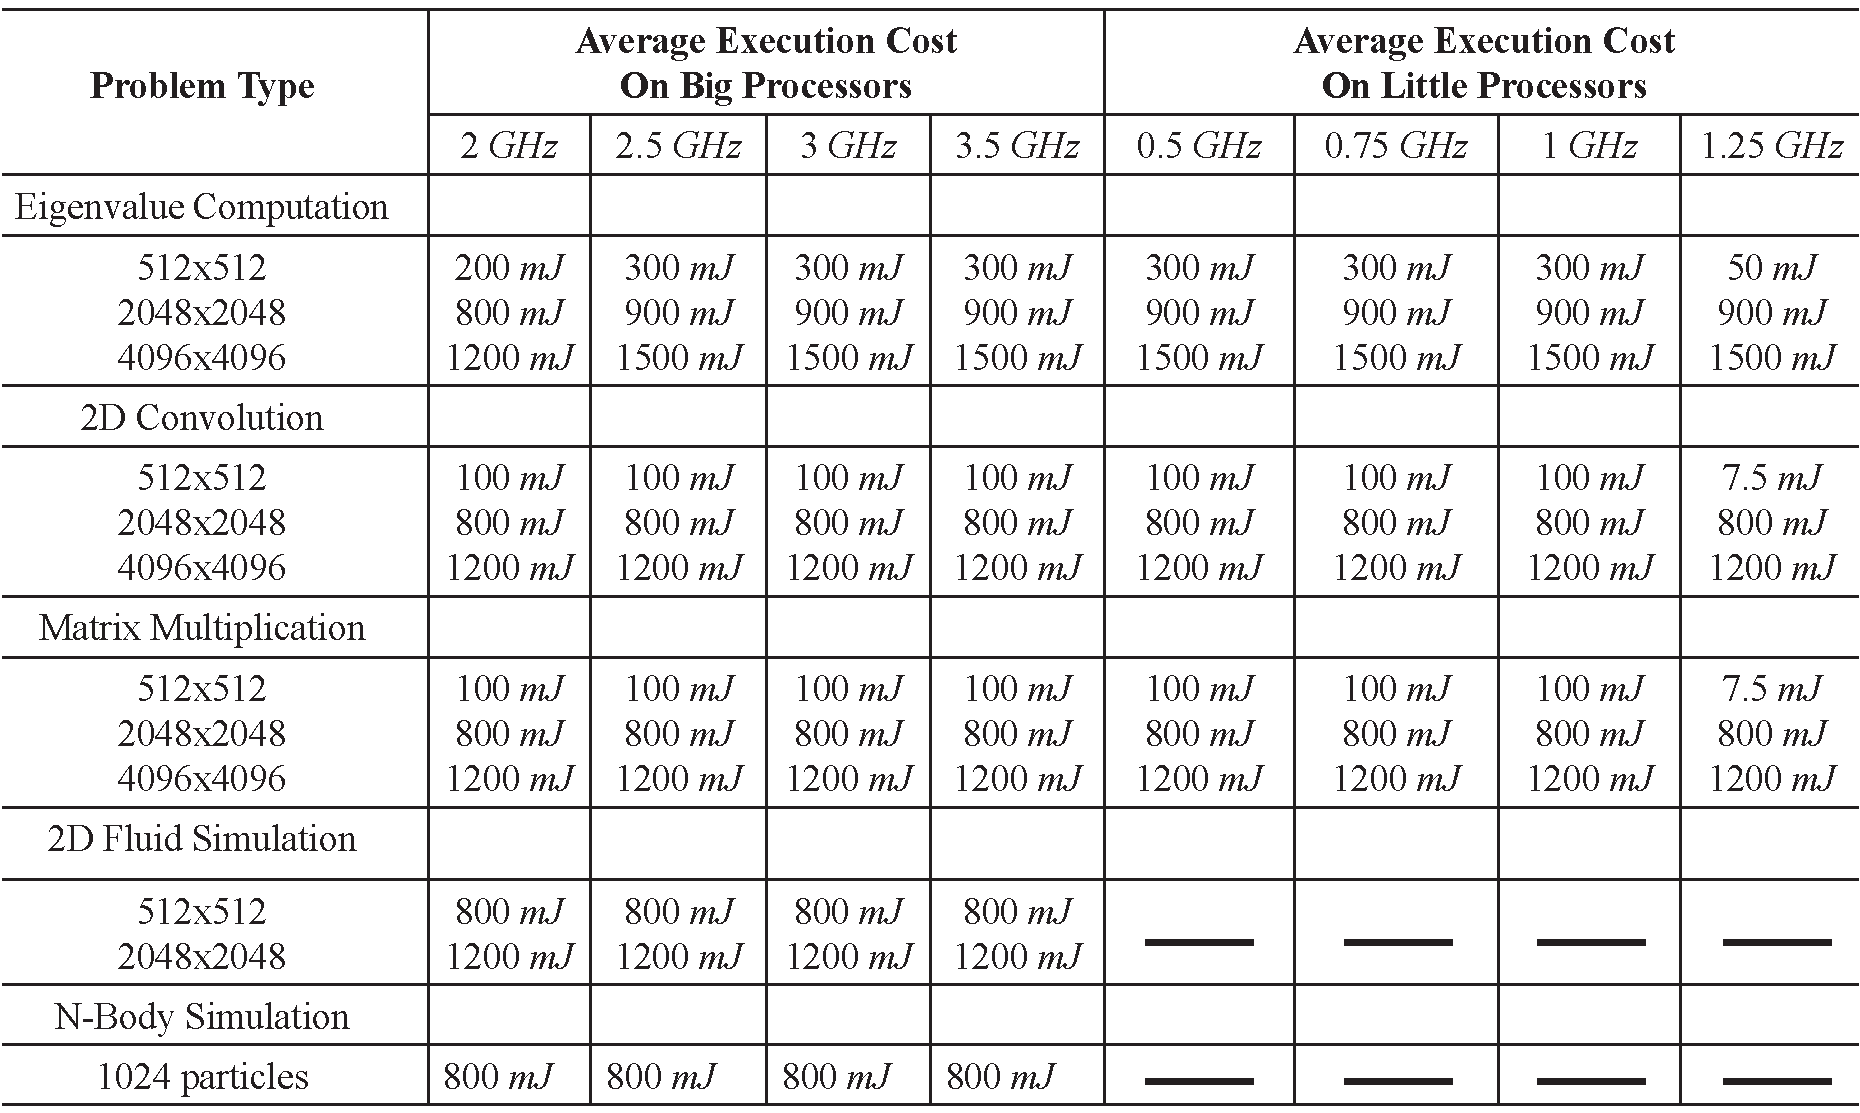
\includegraphics[width=0.65\columnwidth]{images/execution_cost.pdf}
%} \caption{Observed big.LITTLE execution cost under different frequencies.}
%\label{table:herogeneity}
%\end{figure}



 %Figure~\ref{table:herogeneity} summarizes the data we collected for the required energy to execute a job instance on different processors with different frequency settings on an ARM's big.LITTLE platform. 
 As discussed earlier in Section~\ref{sec:hardware}, a key observation seen in Table~\ref{?} is that for certain workloads, the energy consumed on ``big'' processors with the lowest frequency is actually much larger than the energy consumed on ``LITTLE'' processors with the highest frequency. This indicates that if a task is first scheduled on a ``big'' processor to achieve the best  timing performance and then executed with a lowed frequency to save energy (i.e., the current practice), the resulting energy consumption may ironically be much larger than scheduling the task on a ``LITTLE'' processor according to its heterogeneous energy characteristics.  However, this observation does not simply suggest that all workloads shall be first scheduled to ``little'' processors to be energy efficient because (\textit{i}) doing so may cause timing violations due to the overloaded ``LITTLE'' processors, and (\textit{ii}) there also exist tasks whose heterogeneity in terms of the energy characteristics on different processors is rather small. Thus, we argue that the computing capacity provided by different processors to execute a particular task is required to be properly selected to save energy as the heterogeneity of processors arises, which can be further motivated by the following example.

%We illustrate this point by considering the generalized scheduling problem on big.LITTLE heterogeneous multiprocessor platforms, which we now define. Let $J = (r, c^{big}, c^{LITTLE}, d)$ denote a real-time job arriving at time $r$ and needing to execute for $c^{big}$ time units on ``big'' processors or $c^{LITTLE}$ time units on ``LITTLE'' processors by a deadline at time $d$.

%\textbf{The generalized heterogeneous multiprocessor scheduling problem}: Given a real-time instance $I = {J_1, J_2, . . . , J_n}$, and a specific heterogeneous multiprocessor platform~(e.g.~big.LITTLE), determine the smallest $E_{sum}$ such that instance $I$ is feasible upon a platform of total energy consumption $E_{sum}$, in which no job violates its HRT or SRT timing requirement.


\begin{wrapfigure}{r}{0.55\textwidth}
\vspace{-4mm}
\centerline{
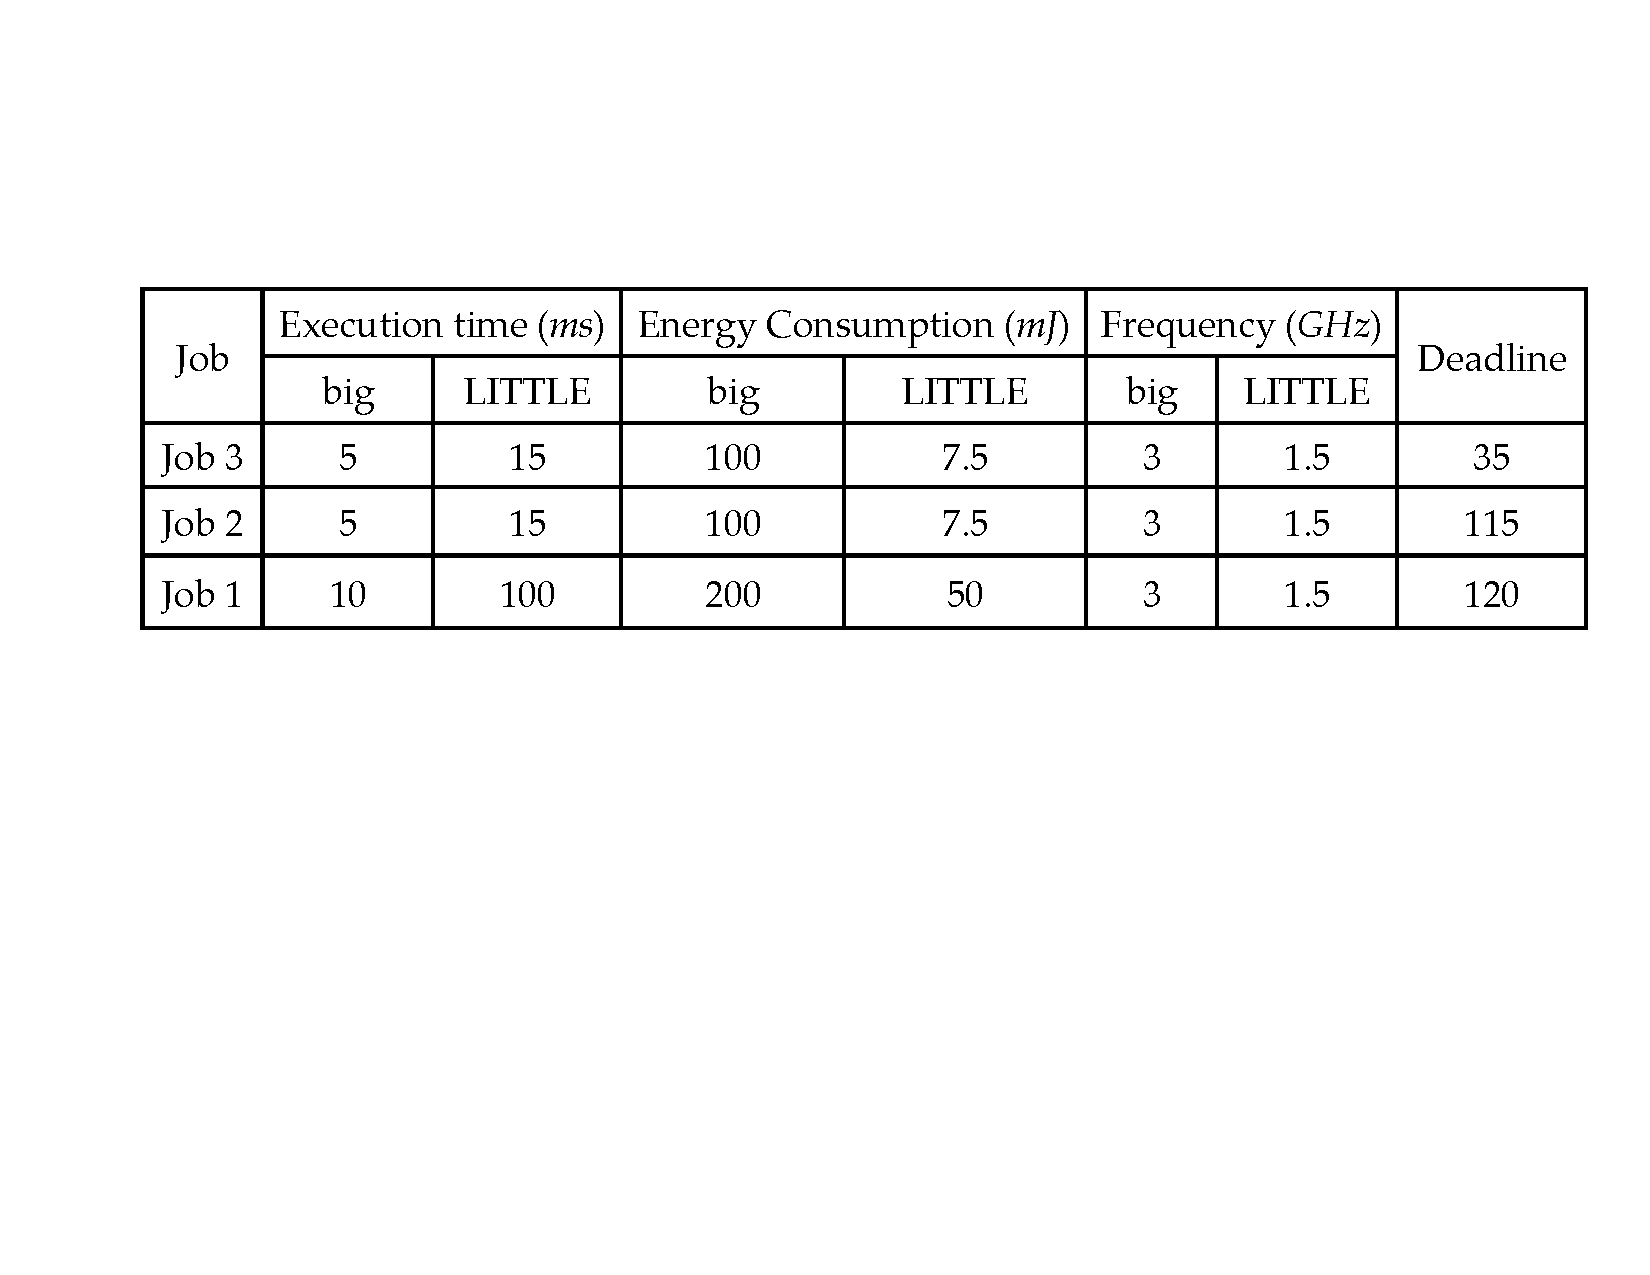
\includegraphics[width=0.55\columnwidth]{images/example_table.pdf}
} \caption{\small An example job set run on  big.LITTLE.}\vspace{-4mm}
\label{fig:big.little}
\end{wrapfigure} \normalsize

\vspace{2mm}
\noindent \textbf{Example.}
An example job set instance is comprised of the following three jobs:
\begin{itemize}
\item $J_1$ = (0, 10, 100, 120); $J_2$ = (0, 5, 15, 115); $J_3$ = (0, 5, 15, 35),
\end{itemize}
 where $J = (r, c^{big}, c^{LITTLE}, d)$ denotes a real-time job arriving at time $r$ and needing to execute for $c^{big}$ time units on ``big'' processors or $c^{LITTLE}$ time units on ``LITTLE'' processors by a deadline at time $d$. 
 The platform associated parameters are shown in Figure~\ref{fig:big.little}. Suppose that we wish to schedule this instance on a big.LITTLE platform in which processor speeds will remain static during run-time (note that we can apply  DVFS on different processors later to further save energy). We consider three different schedulers. The first scheduler is a classical real-time scheduler namely global-early-deadline-first (GEDF), with the resulting schedule shown in Figure~\ref{fig:edf}. Under GEDF, the job with the earliest deadline will be scheduled on an earliest available processor. The GEDF schedule completes all three jobs by their deadlines, but yielding a total energy consumption of 307.5 mJ. Figure~\ref{fig:workconserving} shows a modified work-conserving schedule where job prioritization and core selection are made by considering both timing- and energy-related parameters. Since $J_1$ exhibit the highest degree of heterogeneity in terms of the difference between the energy consumed on two types of processors, we assign the highest priority to $J_1$, the second highest priority to $J_3$, and the lowest priority to $J_2$ (which has the longest deadline). Doing so allows $J_1$ to be allocated to the ``LITTLE'' processor and the resulting energy consumption can be reduced to 250 mJ. Notice that $J_2$ is assigned to the ``big'' processor since this processor idles first at time 5. Under the third scheduler, as shown in Fig.~\ref{fig:optimal}, the energy consumption can be further reduced to 157.5 mJ (which is optimal for this example). This is by employing a non-work-conserving scheduler, which enforces $J_2$ to wait to be scheduled on its favorite processor in terms of energy consumption, even if the unfavorable ``big'' processor becomes idle at time 5.


 
 \begin{figure*}
\centering
\subfloat[]{\label{fig:edf}
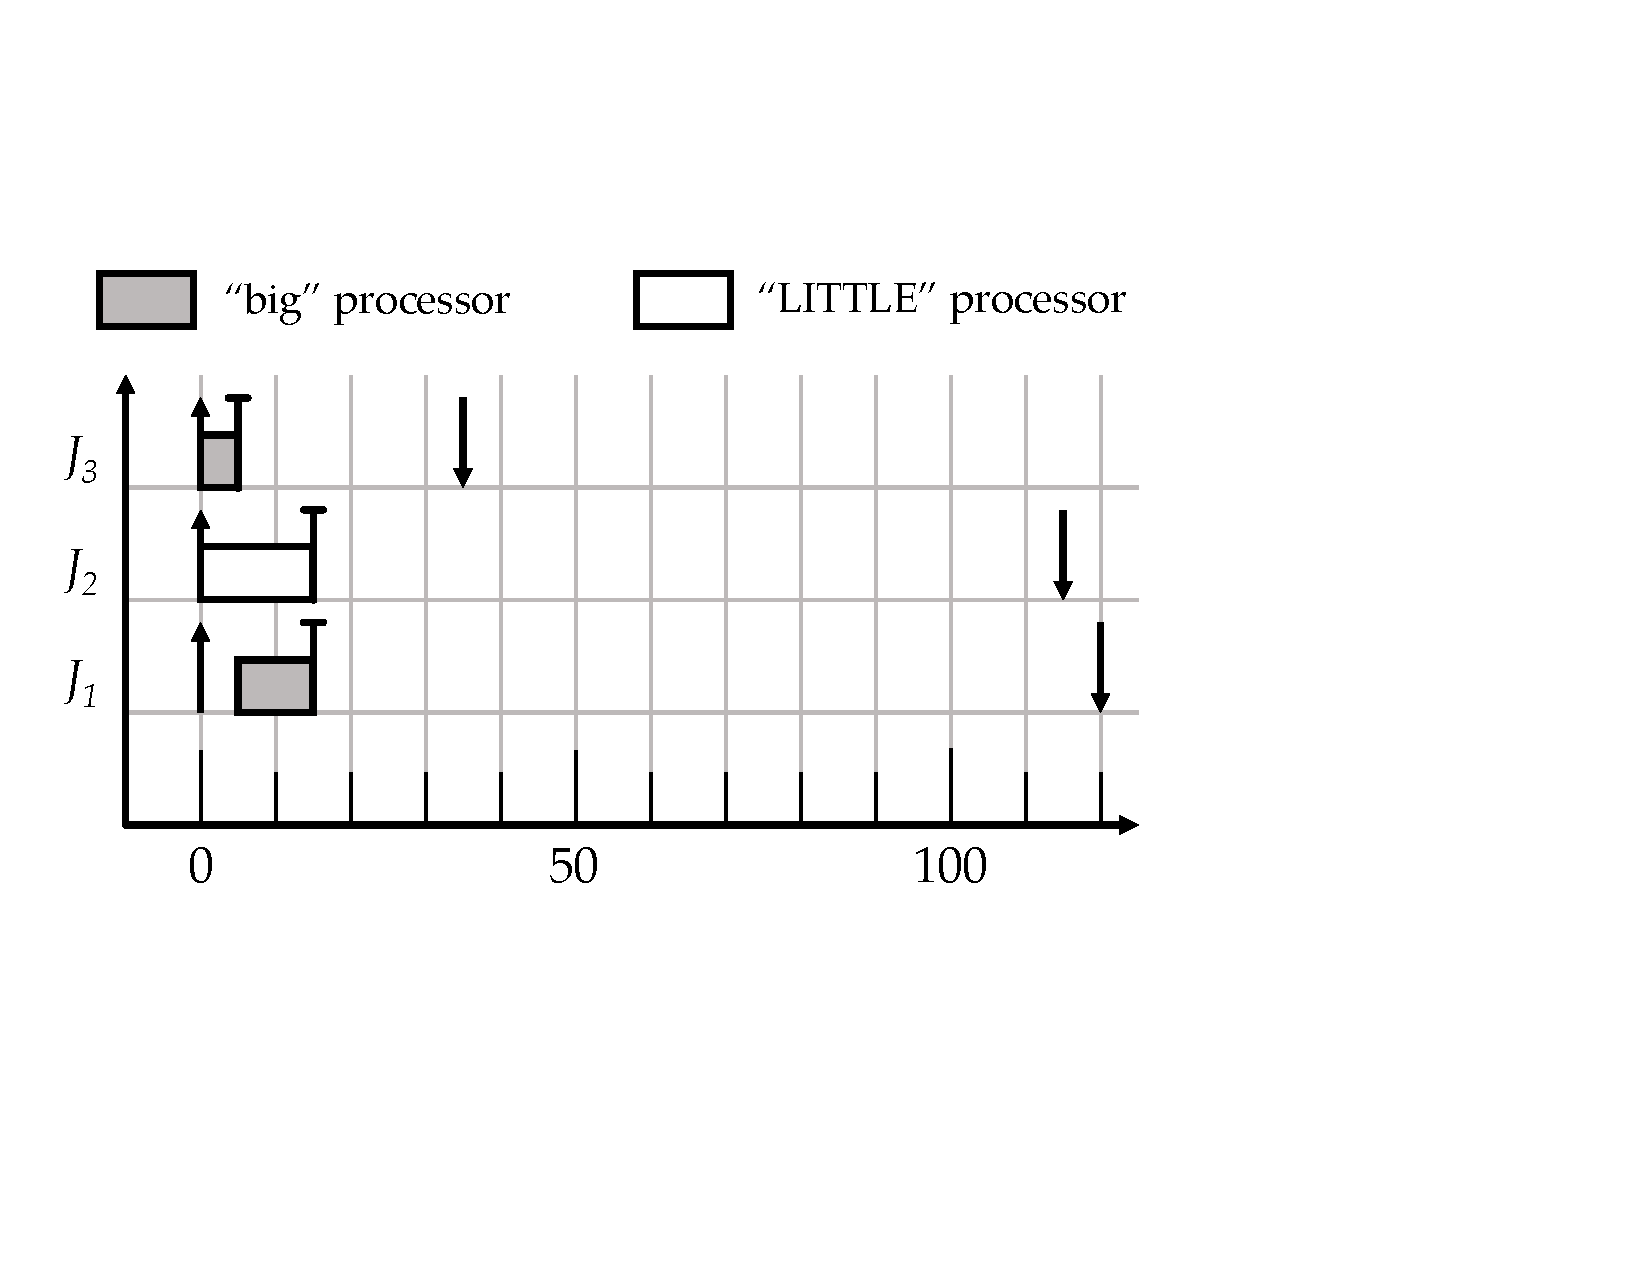
\includegraphics[width=0.32\columnwidth]{images/example_1.pdf}}
\subfloat[]{\label{fig:workconserving}
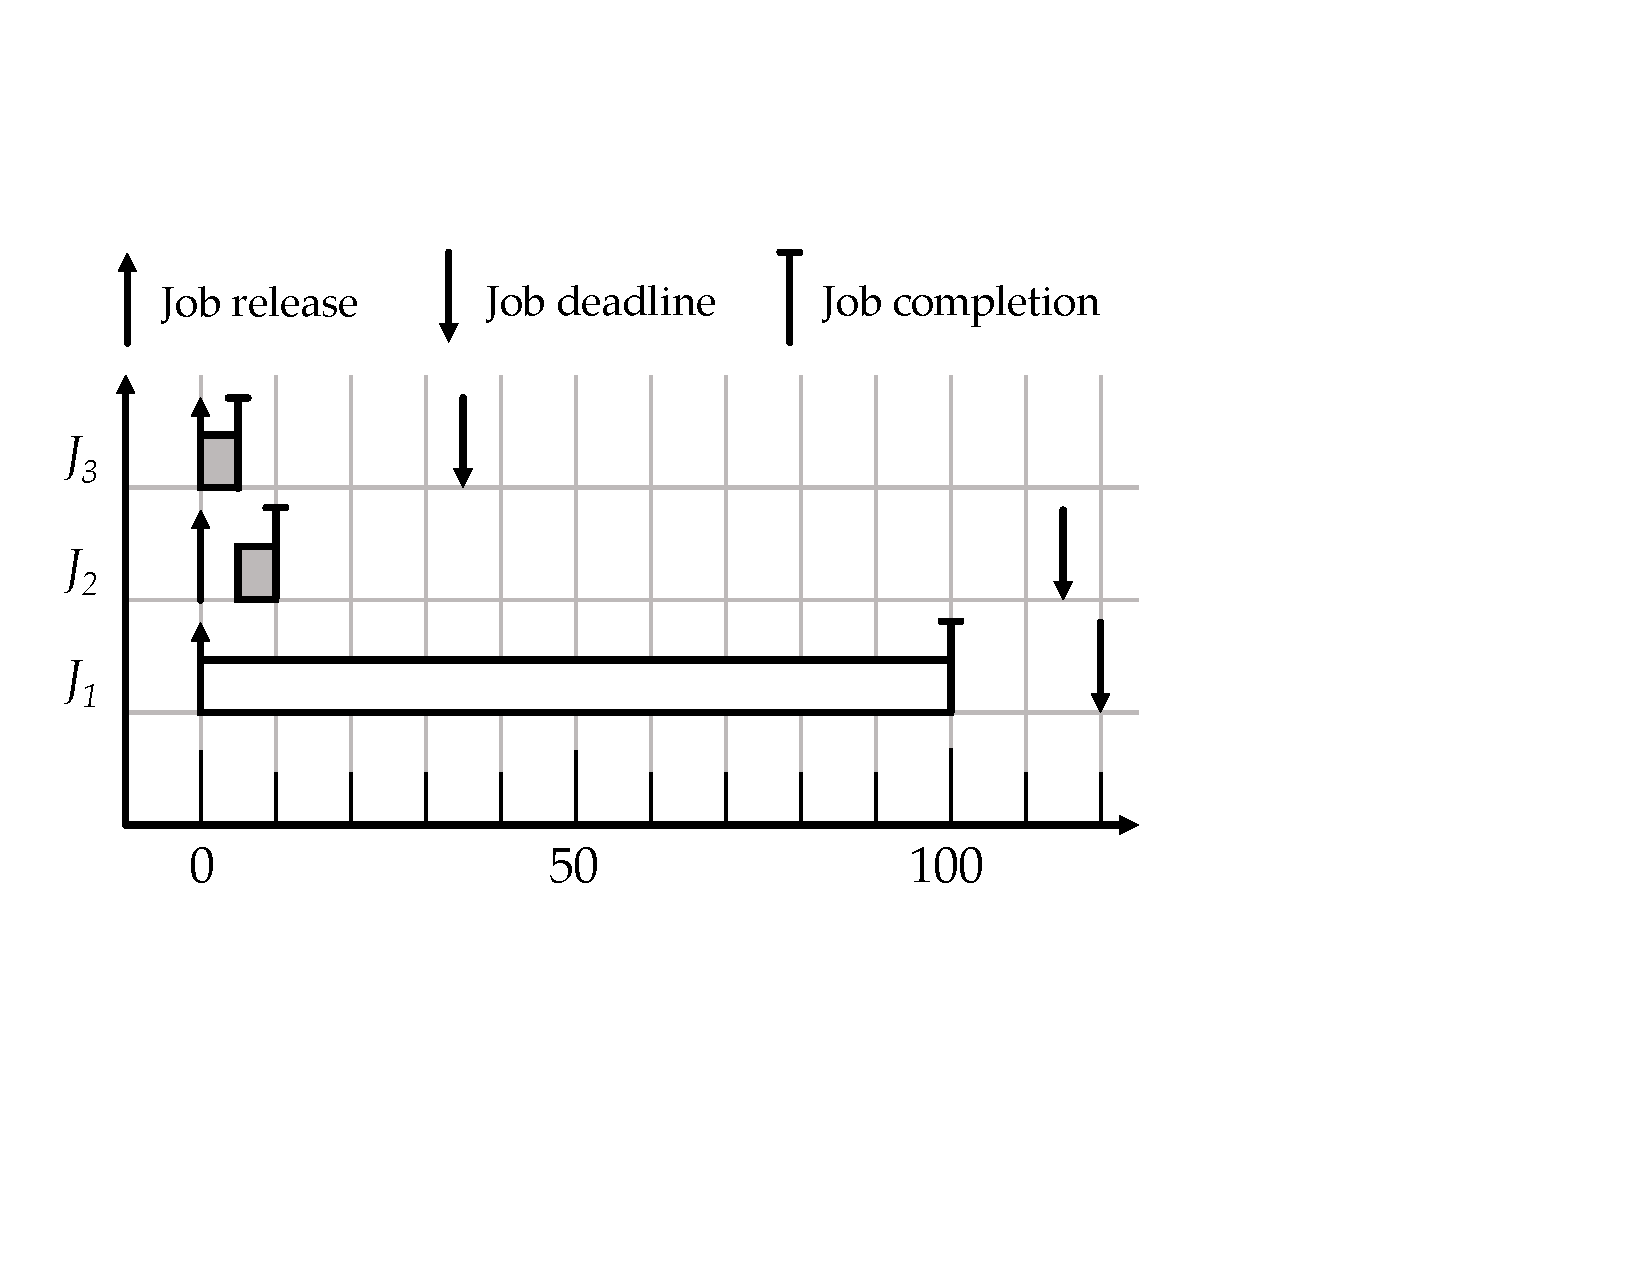
\includegraphics[width=0.32\columnwidth]{images/example_2.pdf}}
\subfloat[]{\label{fig:optimal}
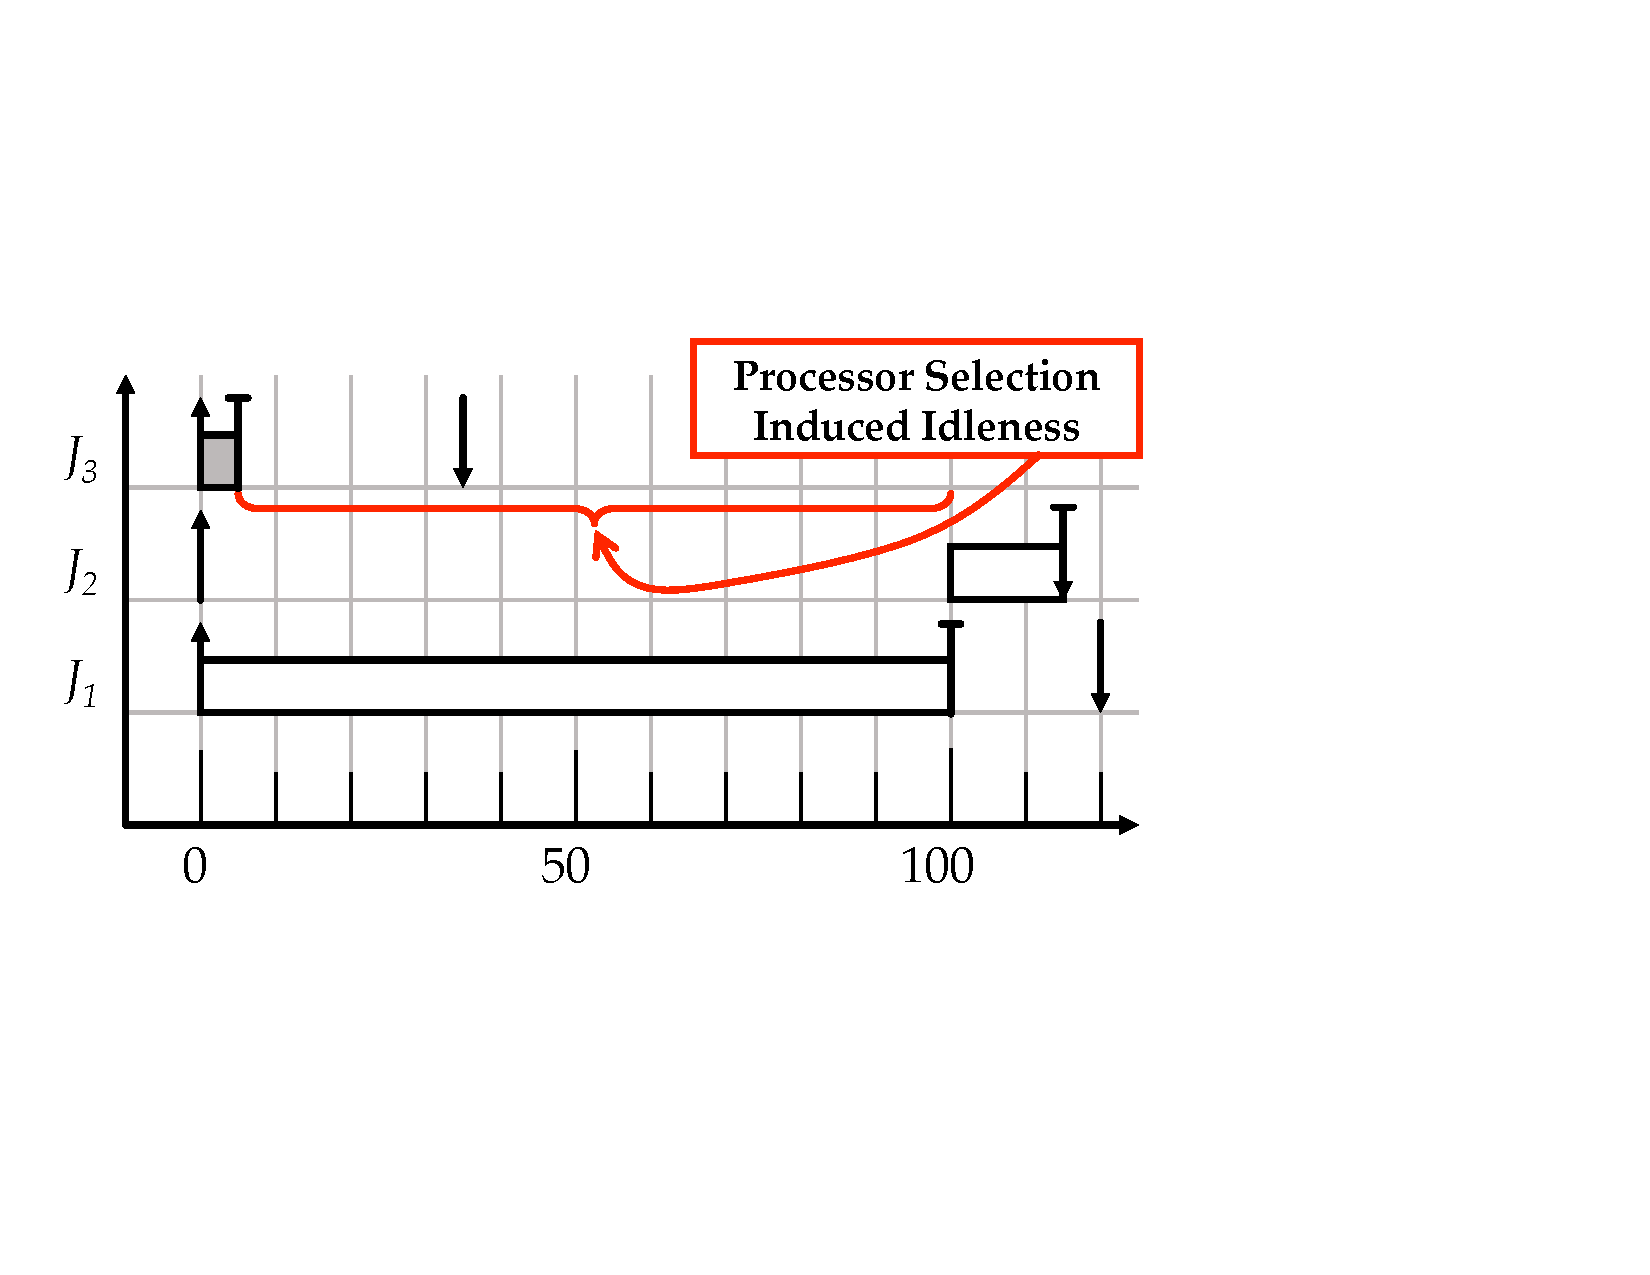
\includegraphics[width=0.32\columnwidth]{images/example_3.pdf}}
\vspace{-2mm}
\caption{\small (a) G-EDF yields $307.5~mJ$; (b) A work-conserving energy-aware scheme yields $250~mJ$; (c) A non-work-conserving energy-aware scheme yields $157.5~mJ$.}\normalsize
\vspace{-2mm}
\end{figure*}

The above example highlights the motivation behind our design of energy-efficient real-time schedulers on heterogeneous platforms, that is, fundamental energy efficiency on heterogeneous platforms can be achieved when a scheduler determines both job prioritization and processor selection by considering tasks' heterogeneous energy characteristics on different processors as ``first-class citizen'' parameters.
% Moreover, as this example shows, there is a non-trivial relationship between the minimum amount of required energy by a real-time instance, and the scheduling method that is feasible to satisfy timing requirements. For simple workloads comprised entirely of a fixed collection of independent jobs (as in the the example above), it may be possible to present this solution space as a collection of simple constraints, and identify optimal solutions using standard optimization techniques. However, the problem becomes considerably more difficult if the instance to be scheduled is represented more succinctly than by enumerating all jobs (e.g., as sporadic tasks). Solving this problem is an essential prerequisite to obtaining optimal or near-optimal energy-efficient implementations of embedded real-time systems. Consequently, one of our major goals is to obtain general solution techniques for solving the problem of real-time task scheduling on a heterogeneous platform that yields the minimum energy consumption.

\vspace{-1mm}
\paragraph{Energy-oriented task prioritization and processor selection schemes.} We propose to investigate a number of potential task prioritization and processor selection schemes that make decisions by considering tasks' heterogeneous energy characteristics. Note that any of these schemes will be viewed as a core component of each different scheduling methodology (e.g., partitioned, clustered, or global scheduling, as will be discussed later in Section~\ref{sec:step1Config}). We will investigate the following two categories of such schemes:

\begin{itemize}
\item[1.] \textbf{Energy-efficient schemes (EES):} We first apply classical real-time task prioritization schemes (e.g., EDF), and then schedule each task to the processor that yields the minimum energy consumption while guaranteeing timing correctness. The tradeoff herein is that applying classical timing-oriented task prioritization may yield tighter schedulability analysis; while applying energy-oriented processor selection may yield better energy efficiency.
\item[2.] \textbf{Energy-aggressive schemes (EAS):} For more aggressive energy savings, we will apply a set of energy-oriented task prioritization rules, and then schedule each task to the processor that yields the minimum energy consumption while guaranteeing timing correctness. We propose to consider the following energy-oriented task prioritization rules: (\textit{i}) largest-energy-heterogeneity-ratio-first: tasks with the higher energy heterogeneity ratio will be assigned higher priorities, where a task's energy heterogeneity ratio is defined to be  the energy consumed for running it on a ``big'' processor divided by the energy consumed for running it on a ``LITTLE'' processor. The intuition is that more energy would be wasted if a task with a higher energy heterogeneity ratio is scheduled to an unfavorite type of processor in terms of energy. (\textit{ii}) largest-energy-difference-first: tasks with larger energy difference values will be assigned higher priorities, where a task's energy difference is defined to be the difference between the energy consumed for running it on a ``big'' processor and a ``LITTLE'' processor. (\textit{iii}) largest-energy-timing-ratio-first: tasks with higher energy-timing ratio will be assigned higher priorities, where a task's energy-timing ratio is defined to be the minimum value between the energy consumed for running it on either a ``big'' or a ``LITTLE'' processor divided by the task's relative deadline.
\end{itemize}

We will discuss next how to incorporate the above energy-oriented task prioritization and processor selection schemes into the large solution space.

\subsubsection{Identifying Energy-Efficient Configurations that Guarantee Timing}
\label{sec:step1Config}

We plan to devise energy-oriented real-time resource allocation methods and the corresponding HRT and SRT schedulability tests that can be applied on heterogeneous computing platforms. These tests will account for runtime system overhead incurred under different methods.

\paragraph{DVFS-based approaches.} The basic resource allocation methods that we believe will be the most fruitful is to apply DVFS combined with energy-oriented scheduling to reduce energy consumption. This is motivated by our experimental data showing that for many applications, scaling down the frequency yields considerably more energy saving than race-to-idle (as discussed in Section~?where?). The solution space for defining such resource allocation methods is vast. As noted earlier, processor capacity can be allocated on a partitioned, clustered, or global basis. For each allocation methodology, the three DVFS methods can be applied (as discussed in Section~\ref{sec:relatedwork}).

\begin{wrapfigure}{R}{0.45\textwidth}
\vspace{-3mm}
\centerline{
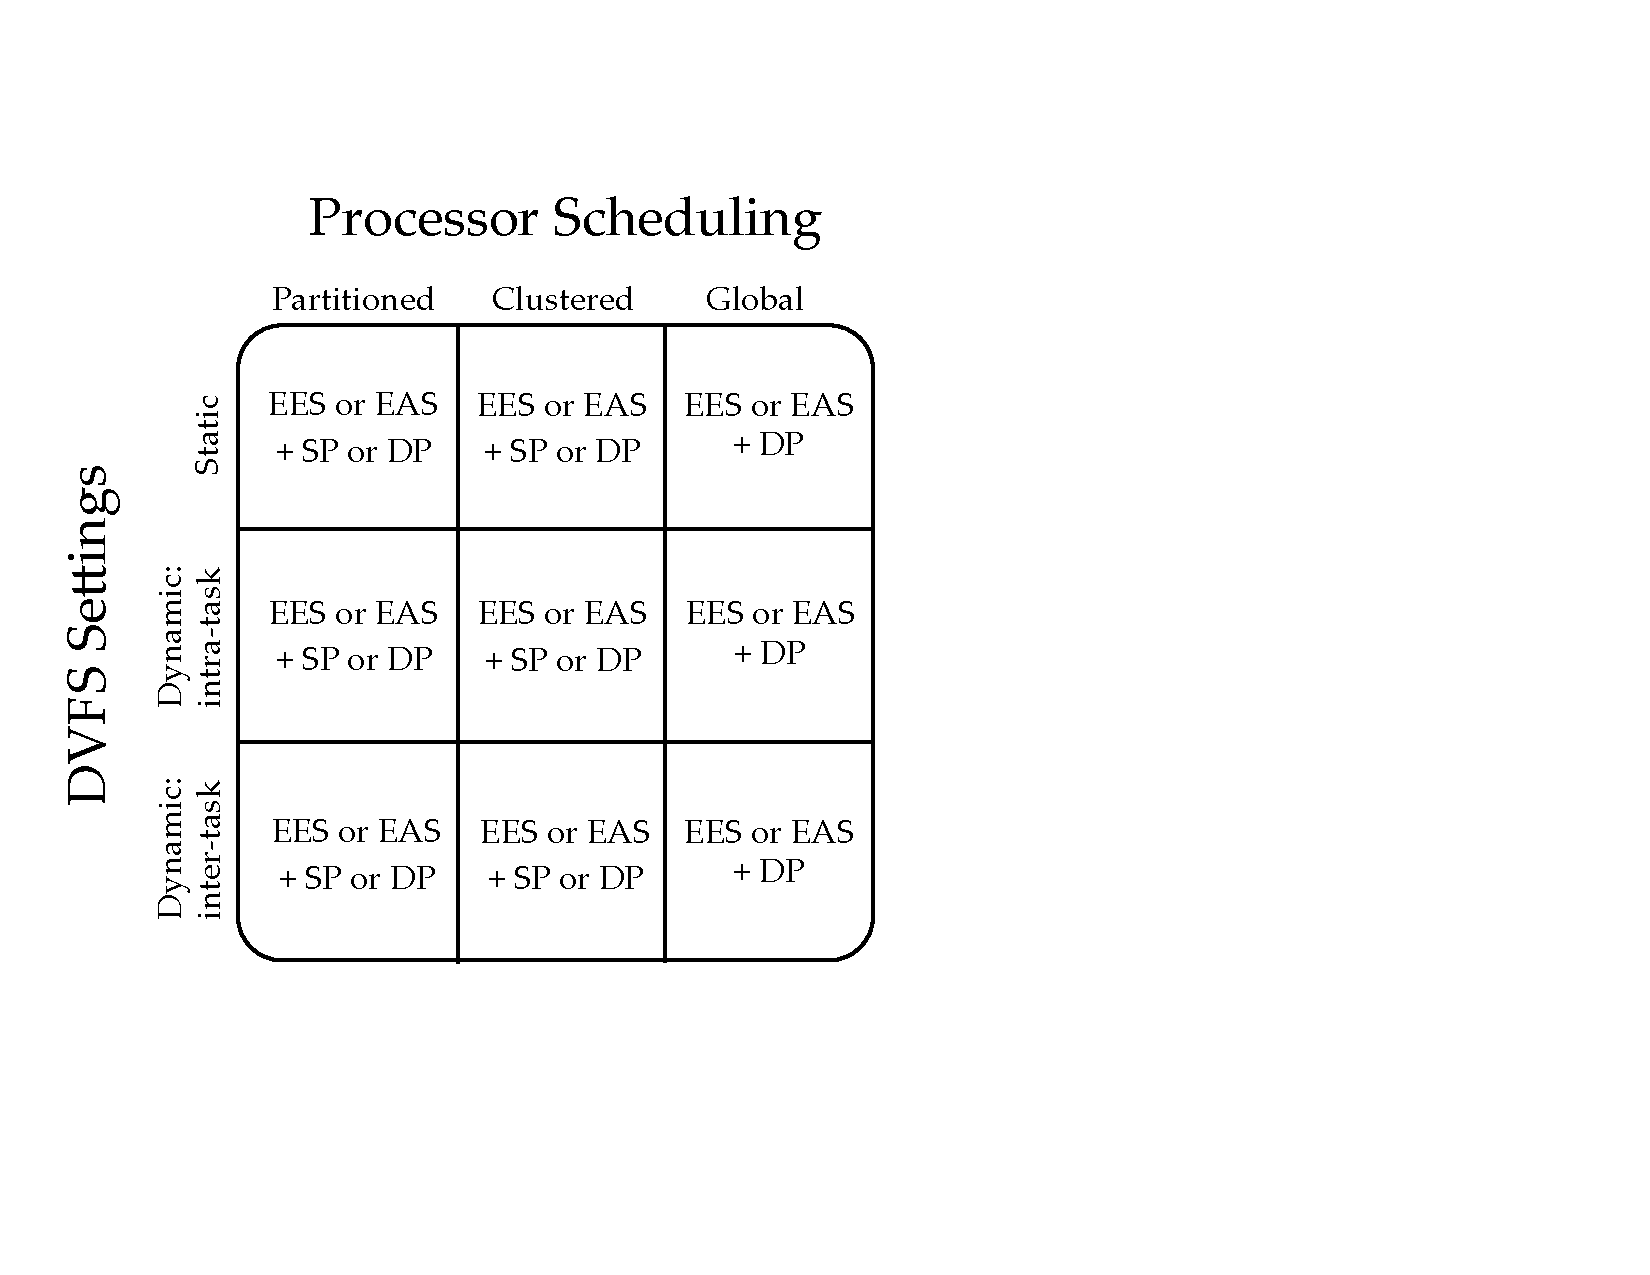
\includegraphics[width=0.42\textwidth]{images/configurations.pdf}
} \caption{\small Processor scheduling and DVFS settings under either fixed-priority (FP) or dynamic-priority (DP) EES and EAS scheduling schemes.}\normalsize
\label{fig:configurations}
\end{wrapfigure}

Fig. 4 depicts the various configurations that result under dynamic-priority or fixed-priority EES and EAS scheduling algorithms (as defined in Section~\ref{sec:step1Motivation}) and indicates DVFS methods that can be used to support each option. For example, when processors are globally managed, capacity can be allocated using dynamic-priority EES with processing frequency controlled by the static DVFS method.  
 Each configuration may have its benefits. For example, as noted earlier, partitioned approaches generally perform well in HRT domains, while global approaches typically perform better in SRT domains. Also note that we do not intend to investigate static-priority approaches under global scheduling, as previous works~\cite{?} have shown that such approaches suffer from significant pessimism in terms of capacity loss on multiprocessor platforms.

While  Figure~\ref{fig:configurations} implies that there are only nine different scheduler configurations, each configuration can be further specialized. For instance, a single ``big'' processor does not necessarily need to be bound to a single ``LITTLE'' processor under clustered scheduling. Instead, a single ``big'' processor could be clustered along with several ``LITTLE'' processors. However, this minor change yields new challenges when we assign tasks to processors, since the symmetric processor structure (i.e., one ``big'' and one ``LITTLE'' processor) now changes to an asymmetric one (i.e., one ``big'' and multiple ``LITTLE'' processors). This change forces the consideration of other alternatives. We have identified over twenty possible big/LITTLE scheduling/organizational combinations for dynamic-priority systems alone. The situation is similar for static-priority systems. Matters are further complicated by other factors. For example, HRT and SRT systems are subject to different schedulability analysis. Finally, to be practicably applicable, schedulability tests must be augmented to account for system overheads such as OS activities and cache-related preemption and migration costs. %For example, global approaches may be sound in theory but suffer in practice due to frequent job preemption and migrations. 
 The proper accounting of such overheads is extraordinarily tedious as we experienced in our previous works~\cite{?}. The major goal in Part 1 of this project is to sift through all of these analysis alternatives, devise the tightest schedulability analysis that is practicably possible for each alternative. The most energy-efficient ones among these alternatives will also be identified through implementation and extensive evaluation (as detailed in Sections~\ref{sec:implementation} and \ref{sec:evaluation}). 




\paragraph{Multi-frequency scheduling heuristics.}


\paragraph{Non-DVFS-based energy saving approaches.}

